\chapter{Introduction}
\textit{
    ``It [The Present Wrapping Problem] is a common practice that a private business rewards its loyal clients with presents, which are typically wrapped in a costly
    corporate paper covered with the logo of the business. Imagine that you work for such a business which wants to limit the overall amount of paper that can be used for this purpose,
    in order to reduce the associated expenses." \cite{project}
}
\\

In the following report we describe our solutions to the proposed problem.
We develop many strategies exploting different techniques such as \textbf{Constraint Progamming \textit{(CP)}},
\textbf{Satisfiability Modulo Theories \textit{(SMT)}} and also \textbf{Boolean Satisfiability \textit{(SAT)}}.
\\
The problem is a derivation of the general problem called as \textbf{Bin Packing Problem} \cite{binpack}, where a certain ammount of blocks must fit
in a bounded weighted space, without overlapping each other.
In this particular case, our blocks are represented by presents belonging a 2D discrete space, represented by the gift paper sheet.
Our target is to check if a given amount of presents, with certain dimensions, can fit into a fixed size paper sheet. 

\begin{figure}
	\centering
	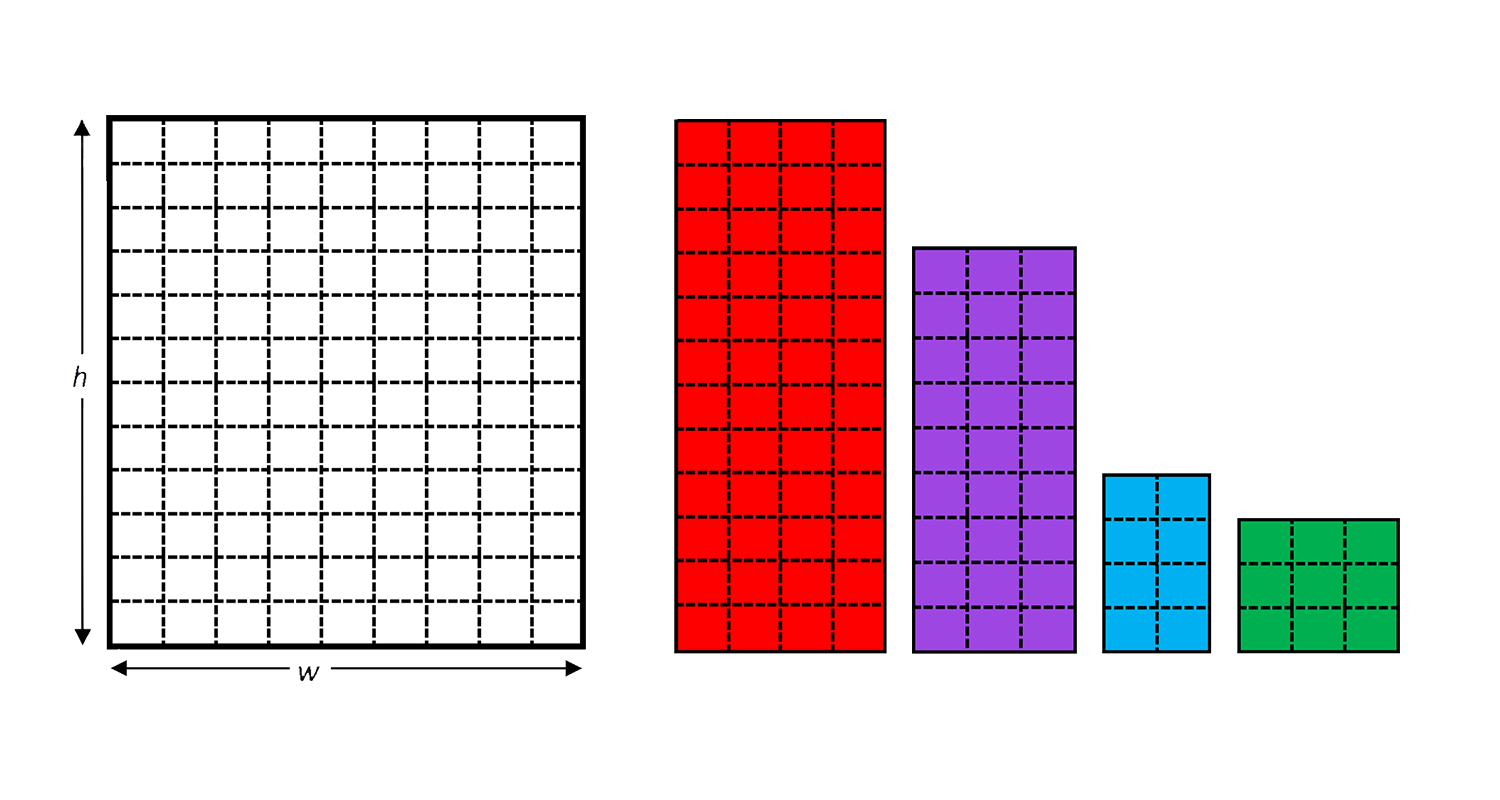
\includegraphics[width=\textwidth]{images/input_problem.png}
	\caption{Example of an instance of a problem with paper and blocks (presents)}
	\label{fig:overlaps}
\end{figure}

\begin{figure}
	\centering
	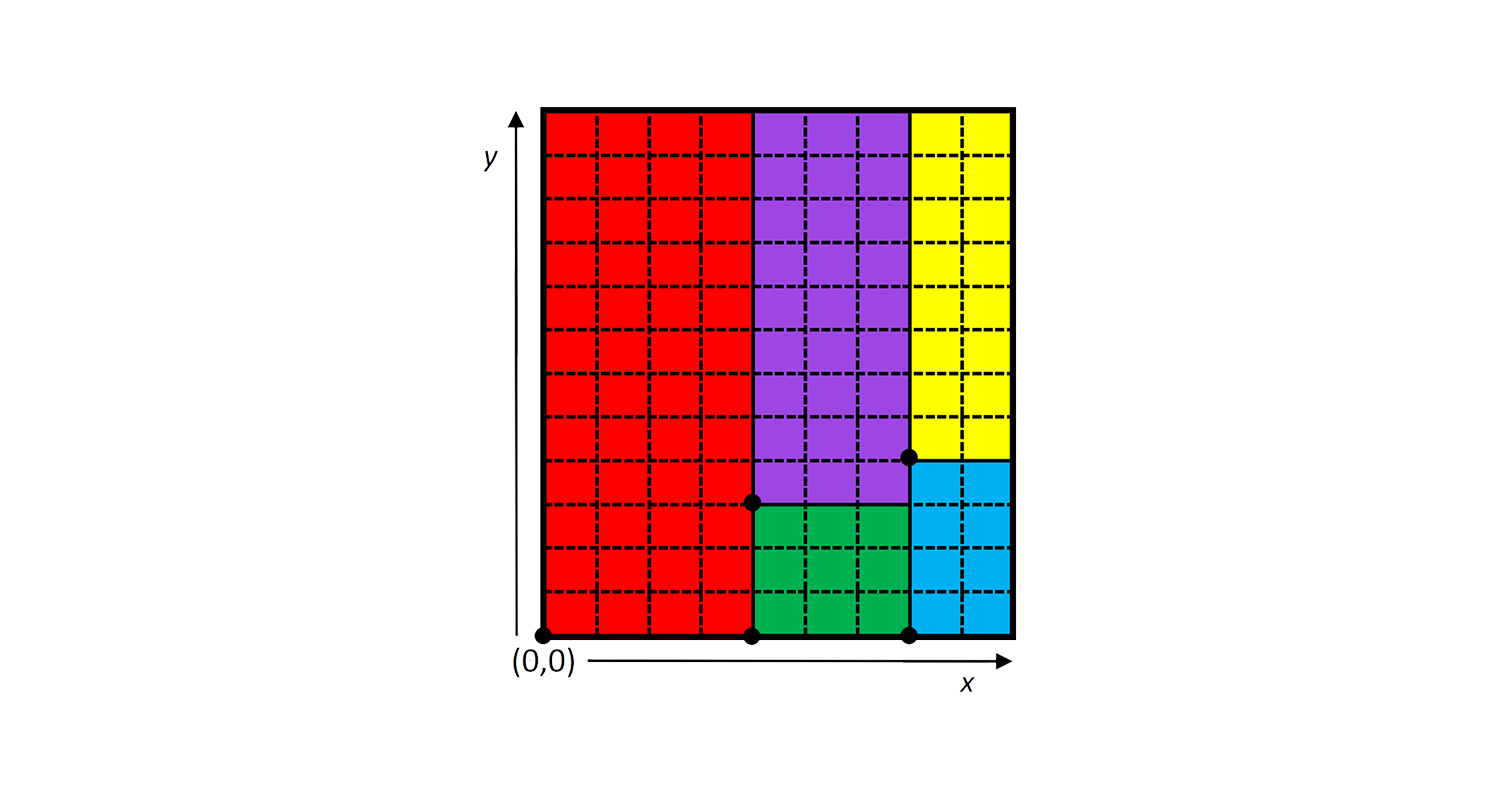
\includegraphics[width=\textwidth]{images/solved_problem.png}
	\caption{A possible solution of the instance shown above}
	\label{fig:overlaps}
\end{figure}